\documentclass[12pt]{article}
\usepackage[english]{babel}
\usepackage[utf8]{inputenc}
\usepackage[english]{babel}
\usepackage[a4paper, total={7.25in, 9.5in}]{geometry}
\usepackage{tikz-feynman}
\tikzfeynmanset{compat=1.0.0} 
\usepackage{subcaption}
\usepackage{float}
\floatplacement{figure}{H}
\usepackage{simpler-wick}
\usepackage{mathrsfs}  
\usepackage{dsfont}
\usepackage{relsize}
\usepackage{tikz-cd}
\DeclareMathAlphabet{\mathdutchcal}{U}{dutchcal}{m}{n}

\usepackage{cancel}



\newcommand{\field}{\hat{\Phi}}
\newcommand{\dfield}{\hat{\Phi}^\dagger}
 
\usepackage{amsthm, amssymb, amsmath, centernot}
\usepackage{slashed}
\newcommand{\notimplies}{%
  \mathrel{{\ooalign{\hidewidth$\not\phantom{=}$\hidewidth\cr$\implies$}}}}
 
\renewcommand\qedsymbol{$\square$}
\newcommand{\cont}{$\boxtimes$}
\newcommand{\divides}{\mid}
\newcommand{\ndivides}{\centernot \mid}

\newcommand{\Integers}{\mathbb{Z}}
\newcommand{\Natural}{\mathbb{N}}
\newcommand{\Complex}{\mathbb{C}}
\newcommand{\Zplus}{\mathbb{Z}^{+}}
\newcommand{\Primes}{\mathbb{P}}
\newcommand{\Q}{\mathbb{Q}}
\newcommand{\R}{\mathbb{R}}
\newcommand{\ball}[2]{B_{#1} \! \left(#2 \right)}
\newcommand{\Rplus}{\mathbb{R}^+}
\renewcommand{\Re}[1]{\mathrm{Re}\left[ #1 \right]}
\renewcommand{\Im}[1]{\mathrm{Im}\left[ #1 \right]}
\newcommand{\Op}{\mathcal{O}}

\newcommand{\invI}[2]{#1^{-1} \left( #2 \right)}
\newcommand{\End}[1]{\text{End}\left( A \right)}
\newcommand{\legsym}[2]{\left(\frac{#1}{#2} \right)}
\renewcommand{\mod}[3]{\: #1 \equiv #2 \: \mathrm{mod} \: #3 \:}
\newcommand{\nmod}[3]{\: #1 \centernot \equiv #2 \: mod \: #3 \:}
\newcommand{\ndiv}{\hspace{-4pt}\not \divides \hspace{2pt}}
\newcommand{\finfield}[1]{\mathbb{F}_{#1}}
\newcommand{\finunits}[1]{\mathbb{F}_{#1}^{\times}}
\newcommand{\ord}[1]{\mathrm{ord}\! \left(#1 \right)}
\newcommand{\quadfield}[1]{\Q \small(\sqrt{#1} \small)}
\newcommand{\vspan}[1]{\mathrm{span}\! \left\{#1 \right\}}
\newcommand{\galgroup}[1]{Gal \small(#1 \small)}
\newcommand{\bra}[1]{\left| #1 \right>}
\newcommand{\Oa}{O_\alpha}
\newcommand{\Od}{O_\alpha^{\dagger}}
\newcommand{\Oap}{O_{\alpha '}}
\newcommand{\Odp}{O_{\alpha '}^{\dagger}}
\newcommand{\im}[1]{\mathrm{im} \: #1}
\renewcommand{\ker}[1]{\mathrm{ker} \: #1}
\newcommand{\ket}[1]{\left| #1 \right>}
\renewcommand{\bra}[1]{\left< #1 \right|}
\newcommand{\inner}[2]{\left< #1 | #2 \right>}
\newcommand{\expect}[2]{\left< #1 \right| #2 \left| #1 \right>}
\renewcommand{\d}[1]{ \mathrm{d}#1 \:}
\newcommand{\dn}[2]{ \mathrm{d}^{#1} #2 \:}
\newcommand{\deriv}[2]{\frac{\d{#1}}{\d{#2}}}
\newcommand{\nderiv}[3]{\frac{\dn{#1}{#2}}{\d{#3^{#1}}}}
\newcommand{\pderiv}[2]{\frac{\partial{#1}}{\partial{#2}}}
\newcommand{\fderiv}[2]{\frac{\delta #1}{\delta #2}}
\newcommand{\parsq}[2]{\frac{\partial^2{#1}}{\partial{#2}^2}}
\newcommand{\topo}{\mathcal{T}}
\newcommand{\base}{\mathcal{B}}
\renewcommand{\bf}[1]{\mathbf{#1}}
\renewcommand{\a}{\hat{a}}
\newcommand{\adag}{\hat{a}^\dagger}
\renewcommand{\b}{\hat{b}}
\newcommand{\bdag}{\hat{b}^\dagger}
\renewcommand{\c}{\hat{c}}
\newcommand{\cdag}{\hat{c}^\dagger}
\newcommand{\hamilt}{\hat{H}}
\renewcommand{\L}{\hat{L}}
\newcommand{\Lz}{\hat{L}_z}
\newcommand{\Lsquared}{\hat{L}^2}
\renewcommand{\S}{\hat{S}}
\renewcommand{\empty}{\varnothing}
\newcommand{\J}{\hat{J}}
\newcommand{\lagrange}{\mathcal{L}}
\newcommand{\dfourx}{\mathrm{d}^4x}
\newcommand{\meson}{\phi}
\newcommand{\dpsi}{\psi^\dagger}
\newcommand{\ipic}{\mathrm{int}}
\newcommand{\tr}[1]{\mathrm{tr} \left( #1 \right)}
\newcommand{\C}{\mathbb{C}}
\newcommand{\CP}[1]{\mathbb{CP}^{#1}}
\newcommand{\Vol}[1]{\mathrm{Vol}\left(#1\right)}

\newcommand{\Tr}[1]{\mathrm{Tr}\left( #1 \right)}
\newcommand{\Charge}{\hat{\mathbf{C}}}
\newcommand{\Parity}{\hat{\mathbf{P}}}
\newcommand{\Time}{\hat{\mathbf{T}}}
\newcommand{\Torder}[1]{\mathbf{T}\left[ #1 \right]}
\newcommand{\Norder}[1]{\mathbf{N}\left[ #1 \right]}
\newcommand{\Znorm}{\mathcal{Z}}
\newcommand{\EV}[1]{\left< #1 \right>}
\newcommand{\interact}{\mathrm{int}}
\newcommand{\covD}{\mathcal{D}}
\newcommand{\conj}[1]{\overline{#1}}

\newcommand{\SO}[2]{\mathrm{SO}(#1, #2)}
\newcommand{\SU}[2]{\mathrm{SU}(#1, #2)}

\newcommand{\anticom}[2]{\left\{ #1 , #2 \right\}}


\newcommand{\pathd}[1]{\! \mathdutchcal{D} #1 \:}

\renewcommand{\theenumi}{(\alph{enumi})}


\renewcommand{\theenumi}{(\alph{enumi})}

\newcommand{\atitle}[1]{\title{% 
	\large \textbf{Physics GR8048 Quantum Field Theory II
	\\ Assignment \# #1} \vspace{-2ex}}
\author{Benjamin Church }
\maketitle}

\newcommand{\atitleIII}[1]{\title{% 
	\large \textbf{Physics GR8049 Quantum Field Theory III
	\\ Assignment \# #1} \vspace{-2ex}}
\author{Benjamin Church }
\maketitle}

\theoremstyle{definition}
\newtheorem{theorem}{Theorem}[section]
\newtheorem{definition}{definition}[section]
\newtheorem{lemma}[theorem]{Lemma}
\newtheorem{proposition}[theorem]{Proposition}
\newtheorem{corollary}[theorem]{Corollary}
\newtheorem{example}[theorem]{Example}
\newtheorem{remark}[theorem]{Remark}

\begin{document}

\atitle{2}

\section*{Problem 1}

\subsection*{1.}

We define an inner product on homogeneous polynomials of degree $q$ over complex projective space $\CP{1}$ by,
\[ (P_1, P_2) = \frac{1}{\Vol{\C^\times}} \int \frac{\dn{4}{z}}{|z|^{2q + 4}} \conj{P_1(z)} P_2(z) \]
However, due to the Gauge invariance $z \to \lambda z$ for $\lambda \in \C^\times$ we need to perform Gauge fixing to make this integral finite. We can insert the integral,
\[ 1 = \int \frac{\dn{2}{\lambda}}{|\lambda|^2} \delta^2(G(\lambda z)) |\det{\Delta(\lambda z)} |  \]
where $G(z) = 0$ is the Gauge fixing condition and $\Delta \epsilon = \delta_{\epsilon} G$. Making this insertion we can write, 
\begin{align*}
(P_1, P_2) & =  \int \frac{\dn{2}{\lambda}}{|\lambda|^2} \frac{1}{\Vol{\C^\times}}  \int \frac{\dn{4}{z}}{|z|^{2q + 4}} \conj{P_1(z)} P_2(z) \delta^2(G(\lambda z)) |\det{\Delta(\lambda z)} | 
\\
& = \int \frac{\dn{2}{\lambda}}{|\lambda|^2} \frac{1}{\Vol{\C^\times}} \int \frac{\dn{4}{z}}{|z|^{2q + 4}} \conj{P_1(z)} P_2(z) \delta^2(G(z)) |\det{\Delta(z)} | 
\\
& = \int \frac{\dn{4}{z}}{|z|^{2q + 4}} \conj{P_1(z)} P_2(z) \delta^2(G(z)) |\det{\Delta(z)} | 
\end{align*} 
Where I changed variables $\lambda z \to z$ and used the Gauge invariance of the form,
\[ \frac{\dn{4}{\lambda z}}{|\lambda z|^{2q + 4}} \conj{P_1(\lambda z)} P_2(\lambda z) = \frac{\dn{4}{z}}{|z|^{2q + 4}} \conj{P_1(z)} P_2(z) \]
to eliminate the argument $\lambda z$. Furthermore the integral over the invariant measure,
\[ \int \frac{\dn{2}{\lambda}}{|\lambda|^2} \]
cancels the volume of the Gauge group. Now, set $G(z) = z_2 - 1$ such that $\delta_{\epsilon} G = \epsilon z_2$. The determinant of multiplication by $z_2$ equals the volume of the unit square acted on by $z_2$ which is taken to a rotated square with size length $|z_2|$. Thus, $\det{\Delta} = |z_2|^2$. Thus, the inner product becomes,   
\[ (P_1, P_2) =  \int \frac{\dn{4}{z}}{|z|^{2q + 4}} \conj{P_1(z)} P_2(z) \delta^2(z_2 - 1) |z_2|^2  = \int \frac{\dn{2}{z_1}}{(|z_1|^2 + 1)^{q + 2}} \conj{P_1(z_1, 1)} P_2(z_1, 1) \]
For the degree one polynomials $z_1$ and $z_2$ we have,
\begin{align*}
(z_1, z_1) & = \int \frac{|z_1|^2 \dn{2}{z_1}}{(|z_1|^2 + 1)^{3}} = 2 \pi \int_0^\infty \frac{r^3 \d{r}}{(1 + r^2)^3} = \frac{\pi}{2}
\\
(z_1, z_2) & = \int \frac{\conj{z_1} \dn{2}{z_1}}{(|z_1|^2 + 1)^{3}}  = 0
\\
(z_2, z_1) & = \int \frac{z_1 \dn{2}{z_1}}{(|z_1|^2 + 1)^{3}}  = 0
\\
(z_2, z_2) & = \int \frac{\dn{2}{z_1}}{(|z_1|^2 + 1)^{3}} = 2 \pi \int_0^\infty \frac{r \d{r}}{(1 + r^2)^3} = \frac{\pi}{2}
\end{align*}
Thus, if $P_1$ and $P_2$ are general degree one polynomials,
\[ P_1(z) = A_1 z_1 + A_2 z_2 \quad \text{and} \quad P_2(z) = B_1 z_1 + B_2 z_2 \]
then,
\[ (P_1, P_2) = \frac{\pi}{2} \left( \conj{A_1} B_1 + \conj{A_2} B_2 \right) \]

\subsection*{2.}

Now we want to apply the gauge $|z_1|^2 + |z_2|^2 = 1$ and $\Re{z_2} > 0$ and $\Im{z_2} = 0$. To do this write $z_1 = x_1 + i x_2$, $z_2 = x_3 + i x_4$ and choose $G_1(z) = |z_1|^2 + \Re{z_2}^2 - 1$ and $G_2(z) = \Im{z_2}$. Consider,
\[ G_1((1 + \epsilon) z) = ((1 + 2 \epsilon_1 + \epsilon_1^2 + \epsilon_2^2) (x_1^2 + x_2^2) + (x_3 + \epsilon_1 x_3 - \epsilon_2 x_4)^2 - 1 \]
Thus, 
\[ \delta_{\epsilon} G_1(z) = 2 (x_1^2 + x_2^2) \epsilon_1 + 2 x_3^2 \epsilon_1 - 2 x_3 x_4 \epsilon_2 \]
Furthermore,
\[ G_2((1 + \epsilon)z) = x_4 + \epsilon_1 x_4 + \epsilon_2 x_3 \]
and thus,
\[ \delta_{\epsilon} G_2(z) = \epsilon_1 x_4 + \epsilon_2 x_3 \]
Therefore,
\[ \Delta = \begin{pmatrix}
2 x_1^2 + 2 x_2^2 + 2 x_3^2 & - 2 x_3 x_4 
\\
x_4 & x_3 
\end{pmatrix} \]
so the determinant is,
\[ \det{\Delta} = 2 x_1^2 x_3 + 2x_2^2 x_3 + 2 x_3^3 + 2 x_3 x_4^2 \]
Using this notation, the inner product becomes,
\begin{align*}
(P_1, P_2) & = \int \frac{(2 x_1^2 x_3 + 2x_2^2 x_3 + 2 x_3^3 + 2 x_3 x_4^2) \dn{4}{x}}{(x_1^2 + x_2^2 + x_3^2 + x_4^2)^{q + 2}}  \conj{P_1(z)} P_2(z) \delta(x_1^2 + x_2^2 + x_3^2 - 1) \delta(x_4) 
\\
& =  \int \frac{(x_1^2 + x_2^2 + x_3^2 ) \dn{2}{x}}{(x_1^2 + x_2^2 + (\sqrt{1 - |z_1|^2})^2)^{q + 2}}  \conj{P_1(x_1, x_2, x_3, 0)} P_2(x_1, x_2, x_3, 0)  \bigg|_{x_3 = \sqrt{1 - |z_1|^2}}
\\
& = \int \dn{2}{x} \conj{P_1(x_1, x_2, x_3, 0)} P_2(x_1, x_2, x_3, 0) \bigg|_{x_3 = \sqrt{1 - |z_1|^2}}
\end{align*}
where I implemented the condition $\Re{z_2} > 0$ by choosing the positive root of $x_1^2 + x_2^2 + x_3^2 - 1 = 0$ and remembered to divide by $2 x_3$ due to the derivative from the delta factor. Writing this integral in polar coordinates for $z_1$,
\[ (P_1, P_2) = \int_0^1 \int_0^{2 \pi} r \d{\theta} \d{r} \conj{P_1(r \cos{\theta}, r \sin{\theta}, \sqrt{1-r^2}, 0)} P_2(r \cos{\theta}, r \sin{\theta}, \sqrt{1-r^2}, 0) \]
Thus, 
\begin{align*}
(z_1, z_1) & = \int_0^1 \int_0^{2 \pi} r \d{\theta} \d{r} |z_1|^2 = 2\pi \int_0^1 r^3 \d{r} = \frac{\pi}{2}
\\
(z_1, z_2) & = \int_0^1 \int_0^{2 \pi} r \d{\theta} \d{r} \conj{z_1} r  = 0
\\
(z_2, z_1) & = \int_0^1 \int_0^{2 \pi} r \d{\theta} \d{r} r z_1  = 0
\\
(z_2, z_2) & = \int_0^1 \int_0^{2 \pi} r \d{\theta} \d{r} r^3 = 2\pi \int_0^1 r^3 \d{r} = \frac{\pi}{2}
\end{align*}
which is the same result we found earlier. 
Thus, if $P_1$ and $P_2$ are general degree one polynomials,
\[ P_1(z) = A_1 z_1 + A_2 z_2 \quad \text{and} \quad P_2(z) = B_1 z_1 + B_2 z_2 \]
then,
\[ (P_1, P_2) = \frac{\pi}{2} \left( \conj{A_1} B_1 + \conj{A_2} B_2 \right) \]


\subsection*{3.}

Now we will leave the $U(1)$ symmetry of $z \mapsto e^{i \theta} z$ and only gauge fix the $\R^\times$ part of the Gauge group. Consider the Gauge fixing function, $G(z) = |z_1|^2 + |z_2|^2 - w$. For real $\epsilon$,
\[ \delta_{\epsilon} G(z) = 2 \epsilon |z_1|^2 + 2 \epsilon |z_2|^2 = 2 \epsilon |z|^2 \]  
and thus, using our one Gauge fixing condition, the inner product becomes,
\begin{align*} 
(P_1, P_2) & = \frac{1}{\Vol{U(1)}} \int \frac{\dn{4}{z}}{|z|^{2q + 4}} \conj{P_1(z)} P_2(z) \delta^2(G(z)) |\det{\Delta(z)} | 
\\
& = \frac{1}{\pi} \int \frac{\dn{4}{z}}{|z|^{2q + 2}} \conj{P_1(z)} P_2(z) \delta(|z_1|^2 + |z_2|^2 - w) 
\end{align*}
Since this integral is constant with respect to the Gauge fixing condition, we can integrate with respect to the Gauge constant $w$ to get,
\begin{align*}
(P_1, P_2) & = \frac{1}{\pi Z} \int \d{w} w^p e^{-w / \xi} \int \frac{\dn{4}{z}}{|z|^{2q + 4}} \conj{P_1(z)} P_2(z) \delta(|z_1|^2 + |z_2|^2 - w) (|z_1|^2 + |z_2|^2) 
\\
& = \frac{1}{\pi Z} \int \frac{\dn{4}{z}}{|z|^{2q + 2}} \conj{P_1(z)} P_2(z) |z|^{2p} e^{-|z|^2/\xi}
\end{align*}
where,
\[ Z = \int \d{w} w^p e^{-w/\xi} =  \xi^{p+1} \Gamma(p + 1) \]
If we set  $p = q + 1$ then the integral inner product becomes a simple Gaussian with polynomial insertions,
\[ (P_1, P_2) = \frac{1}{\pi Z} \int \dn{4}{z} \conj{P_1(z)} P_2(z) e^{-|z|^2/\xi} \]
Furthermore, 
\[ 
\mathcal{Z} = \int \dn{4}{z} e^{-|z|^2 / \xi} = \pi^2 \xi^2 \]
and then,
\[ \EV{\bar{z}_i z_j} = \frac{1}{\mathcal{Z}} \int \bar{z}_i z_j e^{-|z|^2 / \xi} = \frac{1}{\mathcal{Z}} \int \bar{z}_i z_j e^{-\bar{z}_i \left( \frac{1}{\xi} \delta_{ij} \right) z_j} = \xi \delta_{ij} \]
And therefore, for $q = 1$,
\[ (z_i, z_j) = \frac{\mathcal{Z}}{\pi Z} \EV{\bar{z}_i z_j} = \frac{\pi^2 \xi^2}{\pi \xi^3 2!} \xi \delta_{ij} = \frac{\pi}{2} \delta_{ij} \] 
which reproduces the earlier results. Our general formula becomes,
\[ (P_1, P_2) = \frac{\mathcal{Z}}{\pi Z[q]} \cdot \frac{1}{\mathcal{Z}} \int \conj{P_1(z)} P_2(z) e^{-|z|^2 / \xi} = \frac{\pi}{\xi^q (q+1)!} \sum (\text{Wick Contractions}) \]
Consider a general monomial of the form $P_{ab}(z) = z_1^a z_2^b$ of degree $q = a + b$. I will compute the ``length'' of this general term. Plugging in,
\begin{align*}
(P_{ab}, P_{ab}) = \frac{\pi}{\xi^q (q + 1)!} \sum (\text{Wick Contractions}) = \frac{\pi a! b!}{(q + 1)!} 
\end{align*}
where there are $a!$ ways to contract the $a$ different $z_1, \bar{z}_1$ pairs and $b!$ ways to contract the $b$ different $z_2, \bar{z}_2$ pairs. This works for any degree including $q = 5$. For example,
\begin{align*}
(z_1^5, z_1^5) & = \frac{\pi 5!}{6!} = \frac{\pi}{6}
\\
(z_1^3 z_2^2, z_1^3 z_2^2) & = \frac{\pi 3! 2!}{6!} = \frac{\pi}{60}
\\
(z_1^5, z_1^4 z_2) & = 0
\end{align*}
In the last one we need to Wick contract each $z_1$ with a $\bar{z}_1$ but there are not enough so the $\delta_{ij}$ terms will kill all Wick contractions.  

\section*{Problem 2}
Consider the ``action''
\[ S_0(x,y) = \frac{1}{2 \sigma} (x - y)^2 \]
for which we wish to calculate the expectation of Gauge invariant quantities,
\[ \EV{g} = \frac{1}{Z} \int \d{x} \d{y} e^{-S_0(x,y)} g(x,y) \quad \text{with} \quad Z = \int \d{x} \d{y} e^{-S_0(x,y)} \]
We introduce a ghost $c$ and anti-ghost $\bar{c}$ and an auxiliary field $B$. The BRST operator $Q$ acts via,
\[ Q x = c \quad Q y = c \quad Q c = 0 \quad Q \bar{c} = i B \quad Q B = 0 \]
such that $Q^2 = 0$. Gauge fixing is accomplished by adding a $Q$-exact ghost action $S_G = QF$ for some fixing function $F$ such that the integral becomes well-defined. 


\subsection*{1.}

We will use the trial fixing function,
\[ F = \bar{c} \left( \alpha x + \beta y + \gamma - \tfrac{1}{2} i \xi B \right) \]
such that the ghost action becomes,
\[ S_{G} = QF = \tfrac{1}{2} \xi B^2 + i B\left( \alpha x + \beta y + \gamma \right) - (\alpha + \beta) \bar{c} c \]
Then the characteristic function becomes,
\begin{align*}
Z(\lambda) & = \EV{e^{i \lambda (x - y)}} = \frac{1}{Z} \int \d{x} \d{y} \d{B} \d{\bar{c}} \d{c} e^{- S_0 - S_G + i \lambda (x - y)}
\\
& = \frac{1}{Z} \int \d{x} \d{y} \d{B} \d{c} \d{\bar{c}} \exp{\left[ - \frac{1}{2\sigma}(x - y)^2 - \tfrac{1}{2} \xi B^2 - i B\left( \alpha x + \beta y + \gamma \right) + (\alpha + \beta) \bar{c} c + i \lambda (x - y) \right]}
\end{align*}
First we integrate out the Ghosts,
\[ \int \d{c} \d{\bar{c}} e^{\bar{c} (\alpha + \beta) c}  = (\alpha + \beta) \]
The remaining integral can be evaluated by Mathematica,
\[ \int \d{x} \d{y} \d{B} \exp{\left[ - \frac{1}{2\sigma}(x - y)^2 - \tfrac{1}{2} \xi B^2 - i B\left( \alpha x + \beta y + \gamma \right) + i \lambda (x - y) \right]} = 2\sqrt{2} e^{-\lambda^2 \sigma/2} \pi^{3/2} \sqrt{\sigma} \cdot \frac{1}{\alpha + \beta} \]
and likewise,
\[ Z = (\alpha + \beta) \int \d{x} \d{y} \d{B} \exp{\left[ - \frac{1}{2\sigma}(x - y)^2 - \tfrac{1}{2} \xi B^2 - i B\left( \alpha x + \beta y + \gamma \right)  \right]} = 2\sqrt{2}  \pi^{3/2} \sqrt{\sigma} \]
Therefore,
\[ Z(\lambda) = e^{-\lambda^2 \sigma / 2} \]
which is independent of all the gauge parameters $\alpha, \beta, \gamma, \xi$. 

\subsection*{2.}

However, the function $g(x) = x$ is not Gauge invariant. Correspondingly, the expectation value,
\[ \EV{g} = \frac{1}{Z} \int \d{x} \d{y} \d{B} \d{c} \d{\bar{c}} g(x) \exp{\left[ - \frac{1}{2\sigma}(x - y)^2 - \tfrac{1}{2} \xi B^2 - i B\left( \alpha x + \beta y + \gamma \right) + (\alpha + \beta) \bar{c} c \right]}  = - \frac{1}{\alpha + \beta} \]
which does depend on the choice of BRST gauge fixing. 

\subsection*{3.}

Now we will consider the more general Gauge fixing function,
\[ F = \bar{c} \left( f(x,y) - \tfrac{1}{2} i \xi B \right) \]
Applying $Q$ we get the Ghost action,
\begin{align*}
S_G = QF & = i B \left( f(x,y) - \tfrac{1}{2} i \xi B\right) -\bar{c} \left( \partial_x f + \partial_y f \right) c 
\\
& = \tfrac{1}{2} \xi B^2 + i B f(x,y) -\bar{c} \left( \partial_x f + \partial_y f \right) c 
\end{align*}
The expectation value of any quantity becomes,
\begin{align*}
\EV{g} & = \frac{1}{Z} \int \d{x} \d{y} \d{B} \d{c} \d{\bar{c}} g(x,y) \exp{\left[ - \frac{1}{2 \sigma} (x - y)^2 - \tfrac{1}{2} \xi B^2 - i B f(x,y) + \bar{c} \left( \partial_x f + \partial_y f \right) \bar{c} \right]}
\end{align*}
Now if we get $\xi = 0$ and integrate out $B$ we find,
\begin{align*}
\EV{g} & = \frac{2 \pi}{Z} \int \d{x} \d{y} \d{B} \d{c} \d{\bar{c}} g(x,y) \delta(f(x,y)) \exp{\left[ - \frac{1}{2 \sigma} (x - y)^2 + \bar{c} \left( \partial_x f + \partial_y f \right) \bar{c} \right]}
\end{align*}
Furthermore, integrating out the Ghosts gives,
\begin{align*}
\EV{g} & = \frac{2 \pi}{Z} \int \d{x} \d{y} \d{B}  g(x,y) \delta(f(x,y))  [\det{\Delta}] \exp{\left[ - \frac{1}{2 \sigma} (x - y)^2 \right]}
\end{align*}
where,
\[ \Delta = \left( \pderiv{f}{x} + \pderiv{f}{y} \right) \]
which is exactly the $\delta(f)$ gauge fixing prescription. 
\bigskip\\
Consider the function $f(x,y) = xy - 1$ for Gauge fixing. We have 
\[ \Delta = \left( \frac{f}{x} + \frac{f}{y} \right) = x + y \]
Thus,
\[ \EV{g} = \frac{2 \pi}{Z} \int \d{x} \d{y} g(x,y) (x + y) \delta(xy - 1) \exp{\left[ - \frac{1}{2 \sigma} (x - y)^2 \right]} \]
However, if $xy = 1$ then $(-x)(-y) = 1$ so any solution to $xy - 1 = 0$ is paired with its negative. Since the integrand is odd, this means that $\EV{g} = 0$ identically. The problem is that our choice of Gauge fixing function does not admit a unique solution on each Gauge orbit. Furthermore, the Faddeev-Popov ghost prescription removes the absolute value from the determinant which ensures the positivity of the integral. 

\subsection*{4.}

We now consider an alternative Gauge fixing function,
\[ F = \bar{c} \left( f(x,y) - \tfrac{1}{2} i \xi B \right) \quad \quad f(x,y) = \alpha (x + y) + \lambda (x + y)^3 \]
for $\lambda > 0$, $\alpha > 0$. Then the ghost action becomes,
\[ S_G = QF = \tfrac{1}{2} \xi B^2 + i B \left[ \alpha (x + y) + \lambda (x + y)^3 \right] - \bar{c} \left(2 \alpha + 3 \lambda (x + y)^2 \right) \bar{c} \]
Now we fix,
\[ \alpha = - \frac{1}{\sigma} \quad \quad \xi = \frac{1}{\sigma} \]
and then the gauge-fixed action becomes,
\[ S_{\text{GF}} = S_0  + \frac{1}{2\sigma} B^2 - \frac{i}{\sigma} B \left[ (x + y) + \lambda (x + y)^3 \right]  + \frac{1}{\sigma} \bar{c} \left(2  - 3 (x + y)^2 \right) \bar{c} \]
Integrating out $B$ gives an effective action,
\[ S_{\text{EF}} = S_0 + \frac{1}{2 \sigma} \left[ (x + y) + \lambda (x + y)^3 \right]^2 + \frac{1}{\sigma} \bar{c} \left(2  + \lambda 3 (x + y)^2 \right) \bar{c} \]
This action simplifies to,
\[ S_{\text{EF}} = \frac{1}{\sigma} (x^2 + y^2) + \frac{2}{\sigma} \bar{c} c + \frac{\lambda}{\sigma} (x + y)^4 + \frac{\lambda}{2 \sigma} (x + y)^6 
+ \frac{3 \lambda}{\sigma} \bar{c} (x + y)^2 c \]
which we write as,
\[ S_{\text{FREE}} = \frac{1}{\sigma} (x^2 + y^2) + \frac{2}{\sigma} \bar{c} c \quad \quad S_{\text{INT}} = \frac{\lambda}{\sigma} (x + y)^4 + \frac{\lambda}{2 \sigma} (x + y)^6 
+ \frac{3\lambda}{\sigma} \bar{c} (x + y)^2 c \]
We will need to apply Wick's theorem to these interaction terms so first we need to compute the two-point functions,
\begin{align*}
\EV{x x}_0 & = \frac{1}{Z_0} \int \d{x} \d{y} \d{c} \d{\bar{c}} x^2 e^{- S_{\text{FREE}}}  = \frac{\sigma}{2}  
\\
\EV{y y}_0 & = \frac{1}{Z_0} \int \d{x} \d{y} \d{c} \d{\bar{c}} y^2 e^{- S_{\text{FREE}}}  = \frac{\sigma}{2} 
\\
\EV{c \bar{c}}_0 & = \frac{1}{Z_0} \int \d{x} \d{y} \d{c} \d{\bar{c}} c \bar{c} e^{- S_{\text{FREE}}}  = \frac{\sigma}{2} 
\end{align*}
For bookkeeping I define an effective coupling,
\[ g = \frac{\lambda}{\sigma} \]
In a general Wick contraction at a vertex with $a$ different $x$ lines and $b$ different $y$ lines we get a combinatorial factor of $a! b!$ from different possible orderings of the contractions. Furthermore, the interaction terms contained in $(x + y)^n$ give binomial coefficients which combine with the combinatorial factor of $a! b!$ to give a constant factor of $n!$ at each vertex.  
This gives Feynman rules,
\begin{enumerate}
\item $-4! g$ for each fourth-degree $x$ and $y$ interaction vertex.
\item $-6! g$ for each sixth-degree $x$ and $y$ interaction vertex.
\item $ -6 g$ for each fourth-degree $\bar{c}$-$c$ and $x$ or $y$ interaction vertex.   
\item $\sigma / 2$ for each internal line. 
\item Divide by symmetry factor.
\end{enumerate}
At the two-loop level, we have diagrams,
\begin{align*}
\vcenter{\hbox{
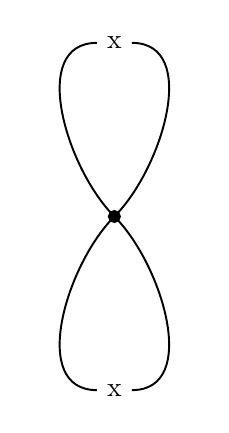
\begin{tikzpicture}[line width=.7pt]
\begin{feynman}
            \vertex (v);
            \vertex[above=2cm of v](t) {x};
            \vertex[below=2cm of v](b) {x};
            \diagram*{
            (v)  -- [out=135,in=180] (t) --[out=0,in=45] (v)
             -- [out=-135,in=180] (b) --[out=0,in=-45] (v)
            };
            \draw[fill=black] (v) circle (2pt);
\end{feynman}
\end{tikzpicture}}}\;
\quad + \quad
\vcenter{\hbox{
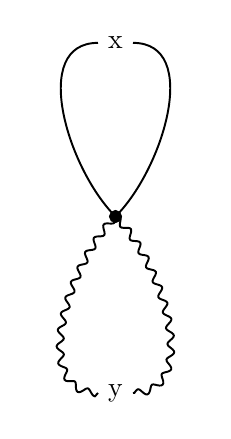
\begin{tikzpicture}[line width=.7pt]
\begin{feynman}
            \vertex (v);
            \vertex[above=2cm of v](t) {x};
            \vertex[below=2cm of v](b) {y};
            \diagram*{
            (v)  -- [out=135,in=180] (t) --[out=0,in=45] (v)
             -- [photon, out=-135,in=180] (b) --[photon, out=0,in=-45] (v)
            };
            \draw[fill=black] (v) circle (2pt);
\end{feynman}
\end{tikzpicture}}}\;
\quad + \quad
\vcenter{\hbox{
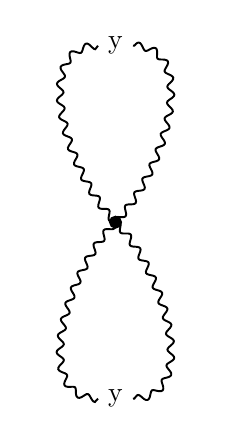
\begin{tikzpicture}[line width=.7pt]
\begin{feynman}
            \vertex (v);
            \vertex[above=2cm of v](t) {y};
            \vertex[below=2cm of v](b) {y};
            \diagram*{
            (v)  -- [photon, out=135,in=180] (t) --[photon, out=0,in=45] (v)
             -- [photon, out=-135,in=180] (b) --[photon, out=0,in=-45] (v)
            };
            \draw[fill=black] (v) circle (2pt);
\end{feynman}
\end{tikzpicture}}}\;
\quad + \quad
\vcenter{\hbox{
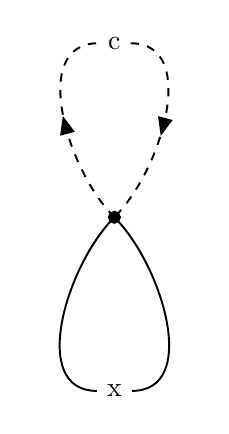
\begin{tikzpicture}[line width=.7pt]
\begin{feynman}
            \vertex (v);
            \vertex[above=2cm of v](t) {c};
            \vertex[below=2cm of v](b) {x};
            \diagram*{
            (v)  -- [charged scalar, out=135,in=180] (t) --[charged scalar, out=0,in=45] (v)
             -- [out=-135,in=180] (b) --[out=0,in=-45] (v)
            };
            \draw[fill=black] (v) circle (2pt);
\end{feynman}
\end{tikzpicture}}}\;
\quad + \quad
\vcenter{\hbox{
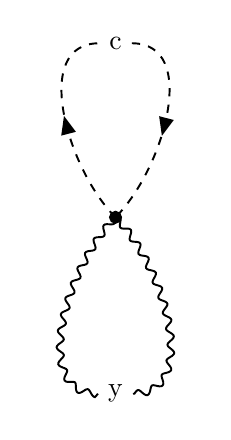
\begin{tikzpicture}[line width=.7pt]
\begin{feynman}
            \vertex (v);
            \vertex[above=2cm of v](t) {c};
            \vertex[below=2cm of v](b) {y};
            \diagram*{
            (v)  -- [charged scalar, out=135,in=180] (t) --[charged scalar, out=0,in=45] (v)
             -- [photon, out=-135,in=180] (b) --[photon, out=0,in=-45] (v)
            };
            \draw[fill=black] (v) circle (2pt);
\end{feynman}
\end{tikzpicture}}}\;
\end{align*}
which, remembering our minus signs for fermion loops, give a total contribution of,
\[ -\frac{4!}{8} \frac{\lambda}{\sigma} \left( \frac{\sigma}{2} \right)^2 - \frac{4!}{4} \frac{\lambda}{\sigma} \left( \frac{\sigma}{2} \right)^2 - \frac{4!}{8} \frac{\lambda}{\sigma} \left( \frac{\sigma}{2} \right)^2 + \frac{6}{2} \frac{\lambda}{\sigma} \left( \frac{\sigma}{2} \right)^2 + \frac{6}{2} \frac{\lambda}{\sigma} \left( \frac{\sigma}{2} \right)^2 = - \left( 3 + 6 + 3 - 6 - 6 \right) \frac{\lambda}{\sigma} \left( \frac{\sigma}{2} \right)^2 = 0 \]
showing that gauge invariance forces the higher-order loop contributions to vanish. 

\subsection*{5.}

We want to compute the cohomology of the operator $Q : \C[x,y,B,c,\bar{c}] \to \C[x,y,B,c,\bar{c}]$. First, note that because $c^2 = \bar{c}^2 = 0$ the ring $R = \C[x,y,B,c,\bar{c}]$ is a finite-dimensional $\C[x,y,B]$-module with basis, $\{1, c, \bar{c}, c \bar{c} \}$. Thus, we can write any element $f$ of $R$ as a sum,
\[ f = f_1 + f_2 c + f_3 \bar{c} + f_4 c \bar{c} \]
where $f_i \in \C[x,y,B]$. We need to know the action of $Q$ on the sub-ring $\C[x,y,B]$. Using the product rule and the fact that $Q B = 0$ we see that if $f \in \C[x,y,B]$ then $Q f = \partial_x f + \partial_y f = \partial f$. I defined the symbol $\partial f$ to be this sum of derivatives. Using this notation, we find that $Q$ acts on the basis as,
\begin{align*}
Q f_1 & = \partial f_1 c
\\
Q f_2 c & = \partial f_2 c^2 = 0
\\
Q f_3 \bar{c} & = \partial f_3 c \bar{c} + i B f_3
\\
Q f_4 c \bar{c} & = \partial f_2 c^2 \bar{c} + f_4 Q c \bar{c} = - i B c f_4  
\end{align*}
Therefore, $Q$ acts on an arbitrary element as,
\[ Qf = i B f_3 + \left( \partial f_1 - i B f_4 \right) c + \partial f_3 c \bar{c} \]
If $Q f = 0$ then we must have $f_3 = 0$ and $\partial_1 - i B f_4 = 0$. Therefore,
\[ \ker{Q} = \{f_1 + f_2 c + f_4 c \bar{c} \mid \partial f_1 = i B f_3 \}  \subset \C[x,y,B,c,\bar{c}] \]
and likewise,
\[ \im{Q} = \{ iB f_3 + \left( \partial f_1 - i B f_4 \right) c + \partial f_3 c \bar{c} \mid f_1, f_3, f_4 \in \C[x,y,B] \} \]
However, the operation $\partial$ is surjective on $\C[x,y,B]$ because $\partial \tfrac{1}{2} x^2 = x$ and $\partial \tfrac{1}{2} y^2 = y$ and $\partial x B = B$ and all products can be accomplished in a similar fashion. Thus, $i B f_3$ can take on any value in $B \C[x,y,B]$ and likewise $\partial f_1 - i B f_4$ can take on any value in $\C[x,y,B]$. Therefore,
\[ \im{Q} = \{ f_1 + f_2 c + f_4 c \bar{c} \mid f_1 \in B \C[x,y,B] \text{ and } \partial f_1 = i B f_4 \} \] 
Consider the map $\Phi : \ker{Q} \to \C[x, y]$ given by sending $f_1 + f_2 c + f_4 c \bar{c}$ to $f_1$ with all $B$ replaced with zeros. This map is $\C[x,y]$-linear and a well-defined homomorphism of $\C$-modules. Furthermore, $f \in \ker{\Phi} \iff f_1 \in B \C[x,y,B] \iff f \in \im{Q}$ so $\ker{\Phi} = \im{Q}$. Furthermore,
take $f \in \ker{Q}$. Suppose that $\partial f_1 \neq 0$ then $\partial f = i B f_3$ for $f_3 \neq 0$ so $f_1 \in B \C[x, y, B]$ meaning that $f \in \im{Q}$ so $\Phi(f) = 0$. Otherwise, $\partial f_1$ and thus $\Phi(f) \in G(\C[x,y]) = \{ \partial g \mid g \in \C[x,y] \} \subset \C[x,y]$. Clearly, this is surjective so $\im{\Phi} = G(\C[x,y])$.
By the first isomorphism theorem,
\[ H(Q) = \ker{Q} / \im{Q} \cong \im{\Phi} = G(\C[x,y]) \subset \C[x,y] \]
which is the ring of gauge-invariant functions $f \in \C[x,y]$. Since $\partial f_1 = 0$ then $f_1$ must be a function of $x - y$. Clearly every function of $x - y$ is gauge-invariant so $G(\C[x,y]) = \C[x-y]$. Finally,
\[ H(Q) = \ker{Q} / \im{Q} \cong \C[x-y] \]
\section*{Problem 3}

Consider a real $N \times N$ symmetric matrix $M$ is drawn randomly from a Gaussian distribution,
\[ P(M) \propto e^{-\frac{1}{2} \Tr{M^2}} \]
If $g(M)$ is an $\mathrm{SO}(N)$-invariant function then its expectation value can be reduced to its expectation value over the distribution of eigenvalues,
\[ \frac{1}{Z} \int \d{M} e^{-\frac{1}{2} \Tr{M^2}} g(M) = \frac{1}{Z'} \int \d{\lambda_1} \cdots \d{\lambda_N} P(\lambda_1, \dots, \lambda_N) g(\lambda_1, \dots, \lambda_N) \]
The action of $\mathrm{SO}(N)$ via $M \mapsto R M R^{\top}$ is a gauge symmetry of the probability function. If $\epsilon$ is a real anti-symmetric $N \times N$ matrix then the infinitesimal gauge transformation is given by $\delta_{\epsilon} M = [\epsilon, M]$. To perform gauge fixing, we require that $M_{ij} = 0$ whenever $i < j$ which forces $M$ to be diagonal because it is symmetric. This fully constrains the gauge. We now define the BRST algebra by introducing a ghost matrix $c$ which is anti-symmetric with Grassmann components, an anti-ghost Grassmann matrix which is upper triangular ($\bar{c}_{ij} = 0$ for $i \ge j$) and an auxiliary bosonic matrix $B_{ij}$ which is also upper triangular. The BRST operator acts as,
\[ QM = [c, M] \quad Qc = c^2 \quad Q \bar{c} = i B \quad QB = 0 \]
We define the Gauge fixing function to be $F = \bar{c}_{ij} M_{ij} = \Tr{\bar{c} M}$ which defines a Ghost action,
\[ S_G = Q F = i B_{ij} M_{ij} - \bar{c}_{ij} \left( c_{ik} M_{kj} - M_{ik} c_{kj} \right)   \]
The Gauge-fixed partition function then becomes,
\[ \EV{g} = \frac{1}{Z} \int \d{M} \d{B} \d{c} \d{\bar{c}} \exp{\left[ -\frac{1}{2} M_{ij} M_{ij} - i B_{ij} M_{ij} + \bar{c}_{ij} \left( c_{ik} M_{kj} - M_{ik} c_{kj} \right) \right] } g(M) \]
First, integrating out $B$ forces,
\begin{align*} 
\EV{g} & = \frac{(2 \pi)^{N(N-1)/2}}{Z} \int \d{M} \d{c} \d{\bar{c}} \delta^{N(N-1)/2}(M_{ij}) \big|_{i < j} \exp{\left[ -\frac{1}{2} M_{ij} M_{ij} + \bar{c}_{ij} \left( c_{ik} M_{kj} - M_{ik} c_{kj} \right) \right] } g(M)
\\
& = \frac{(2 \pi)^{N(N-1)/2}}{Z} \int \d{\lambda_1} \cdots \d{\lambda_N} \d{c} \d{\bar{c}} \exp{\left[ -\frac{1}{2} \sum_{i = 1}^N \lambda_i^2 + \bar{c}_{ij} \left( c_{ij} \lambda_{j} - \lambda_{i} c_{ij} \right) \right] } g(M)
\\
& = \frac{(2 \pi)^{N(N-1)/2}}{Z} \int \d{\lambda_1} \cdots \d{\lambda_N} \d{c} \d{\bar{c}} \exp{\left[ -\frac{1}{2} \sum_{i = 1}^N \lambda_i^2 + \bar{c}_{ij} c_{ij} \left( \lambda_{j} - \lambda_{i} \right) \right] } g(M)
\end{align*}
Now we integrate out the Ghosts,
\begin{align*}
\EV{g} & = \frac{(2 \pi)^{N(N-1)/2}}{Z} \int \d{\lambda_1} \cdots \d{\lambda_N} \det{\left(\delta_{ij = k \ell} \left[ \lambda_j - \lambda_i \right]\right)} \big|_{i < j} \exp{\left[ -\frac{1}{2} \sum_{i = 1}^N \lambda_i^2 \right] } g(M)
\\
& = \frac{(2 \pi)^{N(N-1)/2}}{Z} \int \d{\lambda_1} \cdots \d{\lambda_N} \prod_{i < j} \left[ \lambda_j - \lambda_i \right] \exp{\left[ -\frac{1}{2} \sum_{i = 1}^N \lambda_i^2 \right] } g(M)
\end{align*}
Therefore, up to normalization,
\[ P(\lambda_1, \dots, \lambda_N) \propto \prod_{i < j} \left[ \lambda_j - \lambda_i \right] \exp{\left[ -\frac{1}{2} \sum_{i = 1}^N \lambda_i^2 \right] } \]
Our Gauge fixing prescription is actually to sufficient to fix the form of $M$. We have only fixed $M$ up to permutations of its eigenvectors which explains the odd sign ambiguity in the above expression. To fix this Gauge ambiguity, we choose to order the eigenvalues from smallest to largest such that $P$ is positive. 

\section*{Problem 4}

Consider the Maxwell action,
\[ S_0 = - \frac{1}{4} \int \dn{4}{x} F_{\mu\nu} F^{\mu\nu} \]
with Gauge invariance $A_\mu \mapsto A_\mu + \partial_\mu \chi$ introducing a Gauge freedom in the path integral,
\[ Z = \int \pathd{A} e^{i S_0} \] 
We upgrade this Gauge invariance to a BRST symmetry by introducing a ghost field $c(x)$, anti-ghost field $\bar{c}(x)$, and bosonic field $B$. The BRST variation $\delta_{\eta} = \eta Q$ is actualized by an operator $Q$ acting as,
\[ Q A_\mu = \partial_\mu c \quad Qc = 0 \quad Q \bar{c} = i B \quad QB = 0 \]
We then chose the Gauge fixing function,
\[ F = - i \int \dn{4}{x} \bar{c} \left( \partial_\mu A^\mu + \tfrac{1}{2} B \right) \]
which gives rise to the Ghost action,
\[ S_{\text{GH}} = QF \]
such that the Gauge-fixed action becomes,
\[ S = \int \dn{4}{x} \left( - \tfrac{1}{4} F_{\mu\nu} F^{\mu\nu} + \tfrac{1}{2} B^2 + B \partial_\mu A^{\mu} - i \partial_\mu \bar{c} \partial^\mu c \right) \]

Consider the total variation of the action,
\begin{align*}
\delta S & = \int \dn{4}{x} \left( -\partial_\mu \delta A_\nu ) F^{\mu\nu} + B \delta B + \delta B \partial_\mu A^{\mu} + B \partial_\mu \delta A^{\mu} - i \partial_\mu \delta \bar{c} \partial^\mu c - i \partial_\mu \bar{c} \partial^\mu \delta c \right) 
\end{align*}
Integrating by parts,
\begin{align*}
\delta S & = \int \dn{4}{x} \left( \partial_\mu F^{\mu \nu} - \partial^\nu B \right) \delta A_\nu + \left( B + \partial_\mu A^\mu \right) \delta B - i \partial^2 c \delta \bar{c} + i \partial^2 \bar{c} \delta c
\end{align*}

\subsection*{1.}

We upgrade the BRST symmetry to a local symmetry by making the parameter $\eta$ have spatial dependence. First, we work out the variation of the field strength,
\[ \delta_\eta F_{\mu \nu} = \partial_\mu (\eta \partial_\nu c) - \partial_\nu (\eta \partial_\mu c) = (\partial_\mu \eta) (\partial_\nu c) - (\partial_\nu \eta) (\partial_\mu c) \]
Thus,
\[ \delta_{\eta} (F_{\mu \nu} F^{\mu \nu}) = 2 [(\partial_\mu \eta) (\partial_\nu c) - (\partial_\nu \eta) (\partial_\mu c)] F^{\mu\nu} = 4 (\partial_\mu \eta) (\partial_\nu c) F^{\mu \nu} \]
Furthermore,
\begin{align*}
\delta_{\eta} \left( \partial_\mu \bar{c} \partial^\mu c \right) = \partial_\mu i \eta B \partial^\mu c = i \eta \partial_\mu B \partial^\mu c + i B \partial_\mu \eta \partial^\mu c 
\end{align*}
Therefore,
\begin{align*}
\delta_{\eta} S & = \int \dn{4}{x} \left( - (\partial_\mu \eta) (\partial_\nu c) F^{\mu \nu} + B \partial_\mu (\eta \partial^\mu c) + \eta \partial_\mu B \partial^\mu c + B \partial_\mu \eta \partial^\mu c \right)
\end{align*}
However, 
\[ B \partial_\mu (\eta \partial^\mu c) + \eta \partial_\mu B \partial^\mu c = \partial_\mu (B \eta \partial^\mu c) \]
which can be integrated out to a boundary term. 
Thus,
\[ \delta_{\eta} S = \int \dn{4}{x} \partial_\mu \eta \left( - F^{\mu \nu} \partial_\nu c + B \partial^\mu c \right) \]
and therefore,
\[ j^\mu_{\text{BRST}} = -F^{\mu \nu} \partial_\nu c + B \partial^\mu c \]
Therefore,
\[ \hat{Q} = \int \dn{3}{x} j^0_{\text{BRST}} = \int \dn{3}{x} \left( -F^{0 \nu} \partial_\nu c + B \partial^0 c \right) = \int \dn{3}{x} \left( \vec{E} \cdot \vec{\nabla} c + B \partial_t c \right) \]
Furthermore, we can show that this current is conserved using the classical equations of motion. The Euler-Lagrange equations give,
\[ \partial_\mu F^{\mu \nu} = \partial^\nu B \quad \quad B + \partial_\mu A^\mu = 0 \quad \quad \partial^2 \bar{c} = \partial^2 c = 0 \]
Then consider the divergence of the BRST current,
\begin{align*}
\partial_\mu j^\mu_{\text{BRST}} & = - \partial_\mu F^{\mu \nu} \partial_\nu c - F^{\mu \nu} \partial_\mu \partial_\nu c + \partial_\mu B \partial^\mu + B \partial^2 c
\end{align*}
However, $\partial_\mu \partial_\nu c$ is symmetric and $F^{\mu \nu}$ is anti-symmetric so the second term vanishes. Furthermore, $\partial^2 c = 0$ from the equations of motion so the last term vanishes as well. Thus, using the equations of motion,
\begin{align*}
\partial_\mu j^\mu_{\text{BRST}} & = - \partial_\mu F^{\mu \nu} \partial_\nu c + \partial_\mu B \partial^\mu c
\\
& = - \partial^\nu B \partial_\nu c + \partial_\mu B \partial^\mu c = 0
\end{align*}
so the BRST current and therefore also the BRST charge are conserved.
\subsection*{2.}

The Lagrangian density of this theory is,
\begin{align*}
\lagrange & = - \tfrac{1}{4} F^{\mu \nu} F_{\mu \nu}  + \tfrac{1}{2} B^2 + B \partial_\mu A^{\mu} - i \partial_\mu \bar{c} \partial^\mu c 
\\
& = - \tfrac{1}{2} \partial_\mu A_\nu \partial^\mu A^\nu + \tfrac{1}{2} \partial_\mu A_\nu \partial^\nu A^\mu  + \tfrac{1}{2} B^2 + B \partial_\mu A^{\mu} - i \partial_\mu \bar{c} \partial^\mu c 
\end{align*}
If we vary the time derivatives, $\dot{A}_\mu$, $\dot{c}$, $\dot{\bar{c}}$, we get,  
\begin{align*}
\delta \lagrange & = \left[  \partial^\mu A^t  - \partial^t A^\mu  \right] \delta \dot{A}_\mu + B \delta \dot{A}_t - i (\delta \dot{\bar{c}}) \dot{c} - i \dot{\bar{c}} (\delta \dot{c}) 
\\
& = \left[  \partial^\mu A^t  - \partial^t A^\mu  \right] \delta \dot{A}_\mu + B \delta \dot{A}_t + i \dot{c} (\delta \dot{\bar{c}}) - i \dot{\bar{c}} (\delta \dot{c}) 
\end{align*}
Thus,
\[ \Pi^\mu = \partial^\mu A^t - \partial^t A^\mu + \delta^\mu_t B = F^{\mu t} + \delta^\mu_t B = \vec{E} + \delta^\mu_t B \]
and likewise,
\[ d = - \dot{\bar{c}} \quad \quad  \bar{d} = \dot{c} \]
We then impose the (anti)commutation relations,
\[ \left[ \hat{A}_\mu, \hat{\Pi}^\nu \right] = i \delta_\mu^\nu \quad  \quad \{ \hat{c}, \hat{d} \} = 1 \quad \quad  \{ \hat{\bar{c}}, \hat{\bar{d}} \} = 1 \]
and all other (anti)commutators are zero.
In this canonical variables, the BRST charge becomes simply,
\[ \hat{Q} = \int \dn{3}{x} \hat{\Pi}^\mu \partial_\mu \hat{c} \]

\subsection*{3.}

Written as position-dependent equal-time field (anti)commutation relations we have,
\[ \left[ \hat{A}_\mu(x), \hat{\Pi}^\nu(y) \right] = i \delta_\mu^\nu  \delta^3(x - y) \quad  \quad \{ \hat{c}(x), \hat{d}(y) \} =  \delta^3(x - y) \quad \quad  \{ \hat{\bar{c}}(x), \hat{\bar{d}}(y) \} = \delta^3(x - y) \]
with $\hat{d} = -i \dot{\hat{c}}$. 
Consider the commutators,
\begin{align*}
[ \hat{A}_\mu, \hat{Q} ] & = \int \dn{3}{x} [ \hat{A}_\mu, \hat{\Pi}^\nu ] \partial_\nu c = \int \dn{3}{x} i \delta_\mu^\nu \delta^3(x - y) \partial_\nu c = i \partial_\mu c 
\\
\{ \hat{c}, \hat{Q} \} & = \int \dn{3}{x} \hat{\Pi}^\mu \{ \hat{c}, \partial_\mu c \} = 0
\\
\{ \hat{\bar{c}}, \hat{Q} \} & = \int \dn{3}{x} \hat{\Pi}^\mu \{ \hat{\bar{c}}, \partial_\mu c \} = \int \dn{3}{x} \hat{\Pi}^t \{ \hat{\bar{c}}, \dot{c} \} =  - \int \dn{3}{x} \hat{\Pi}^t \{ \hat{\bar{c}}, \hat{\bar{d}} \} 
\\
& = \int \dn{3}{x} \hat{\Pi}^t  \delta^3(x - y) = \hat{\Pi}^t =  B
\end{align*}
These are identical to the action of the classical BRST operator up to a factor of $i$. 

\subsection*{4.}

We now employ mode expansions of the field operators,
\begin{align*}
A_\mu(x) & = \int \frac{\dn{3}{k}}{(2 \pi)^3} \frac{1}{2 k_0} \left[ a_\mu(k)  e^{-i k x} + a_\mu(k)^\dagger e^{i k x} \right]
\\
B(x) & = i \int \frac{\dn{3}{k}}{(2 \pi)^3} \frac{1}{2 k_0} \left[ k^\mu a_\mu(k) e^{- i k x} - k^\mu a_\mu(k)^\dagger e^{ikx} \right]
\\
c(x) & = \int \frac{\dn{3}{k}}{(2 \pi)^3} \frac{1}{2 k_0} \left[ C(k) e^{ - ikx} + C(k)^\dagger e^{ikx} \right]
\\
\bar{c}(x) & = -i \int \frac{\dn{3}{k}}{(2 \pi)^3} \frac{1}{2 k_0} \left[ \bar{C}(k) e^{- ikx} - \bar{C}^\dagger e^{ikx} \right]
\end{align*}
where the introduced creation and annihilation operators satisfy the (anti)commutation relations,
\[ [a_\mu(k), a_\nu(k')^\dagger] = -\eta_{\mu \nu} 2 k_0 (2 \pi)^3 \delta^3(k - k') \quad \quad \{ C(k), \bar{C}(k')^\dagger \} = \{ \bar{C}(k), C(k')^\dagger \} = 2 k_0 (2 \pi)^3 \delta^3(k - k') \]
Let $\ket{0}$ be the ground state annihilated by $\a_\mu$, $C$, and $\bar{C}$. Consider the state,
\[ \ket{\psi_\mu} = \int \frac{\dn{3}{k}}{(2 \pi)^3} \frac{1}{2 k_0} \tilde{\psi}(k) a_\mu(k)^\dagger \ket{0} \]
where $\tilde{\psi}(k)$ is the momentum space ``wavefunction.'' Then,
\begin{align*}
\inner{\psi_\mu}{\psi_\nu} & = \int \frac{\dn{3}{k}}{(2 \pi)^3} \frac{\dn{3}{k'}}{(2 \pi)^3} \frac{1}{2 k_0} \frac{1}{2 k_0'} \tilde{\psi}_\mu^*(k) \tilde{\psi}_\nu(k') \bra{0} a_\mu(k) a_\nu(k')^\dagger \ket{0} 
\\
& = \int \frac{\dn{3}{k}}{(2 \pi)^3} \frac{\dn{3}{k'}}{(2 \pi)^3} \frac{1}{2 k_0} \frac{1}{2 k_0'} \tilde{\psi}_\mu^*(k) \tilde{\psi}_\nu(k') \bra{0} [ a_\mu(k),  a_\nu(k')^\dagger] \ket{0} 
\\
& = - \int \frac{\dn{3}{k}}{(2 \pi)^3} \frac{\dn{3}{k'}}{(2 \pi)^3} \frac{1}{2 k_0} \frac{1}{2 k_0'} \tilde{\psi}_\mu^*(k) \tilde{\psi}_\nu(k') \eta_{\mu\nu} 2 k_0 (2\pi)^3 \delta^3(k - k')
\\
& = -\int \frac{\dn{3}{k}}{(2 \pi)^3} \frac{1}{2 k_0} \tilde{\psi}_\mu^*(k) \tilde{\psi}_\nu(k) \eta_{\mu\nu} 
\end{align*}
For $\mu = \nu$,
\[ \inner{\psi_\mu}{\psi_\mu} = - \int \frac{\dn{3}{k}}{(2 \pi)^3} \frac{1}{2 k_0} |\psi_\mu(k)|^2 \eta_{\mu \mu} \]
For $\mu = 0$ we have $\eta_{\mu \mu} = 1$ and $|\psi_\mu(k)|^2 \ge 0$ so $\inner{\psi_\mu}{\psi_\mu} < 0$ for $\mu = 0$. Thus, the full Hilbert space admits negative norm states. 

\subsection*{5.}

Now we need to express the BRST operator in terms of the mode expansions. First, we need to compute the mode expansion of the field strength tensor,
\begin{align*}
\partial_\mu A_\nu - \partial_\nu A_\mu & = -i \int \frac{\dn{3}{k}}{(2\pi)^3} \frac{1}{2 k_0} \left[  k_\mu a_\nu(k) e^{-ikx} - k_\mu a_\nu(k)^\dagger e^{ikx} \right] + i \int \frac{\dn{3}{k}}{(2\pi)^3} \frac{1}{2 k_0} \left[ k_\nu a_\mu(k) e^{-ikx}  - k_\nu a_\mu(k)^\dagger e^{ikx} \right] 
\\
& = -i \int \frac{\dn{3}{k}}{(2 \pi)^3} \frac{1}{2 k_0} \left[ (k_\mu a_\nu(k) - k_\nu a_\mu(k) ) e^{-ikx} - (k_\mu a_\nu(k)^\dagger - k_\nu a_\mu(k)^\dagger) e^{ikx} \right]
\end{align*}
Therefore,
\begin{align*}
\hat{Q} & = \int \dn{3}{x} \left( - F^{0 \nu} \partial_\nu c + B \partial^0 c \right)
\\
& = -(-i)^2 \int \dn{3}{x} \int \frac{\dn{3}{k}}{(2 \pi)^3} \frac{\dn{3}{k'}}{(2 \pi)^3}
\frac{1}{2 k_0} \left[ (k_0 a_\nu(k) - k_\nu a_0(k) ) e^{-ikx} - (k_0 a_\nu(k)^\dagger - k_\nu a_0(k)^\dagger) e^{ikx} \right]
\\
& \quad \quad \quad \quad \cdot
\frac{1}{2 k_0'} \left[ k'^\nu C(k') e^{-ik'x} - k'^\nu C(k')^\dagger e^{ik'x}  \right] 
\\
&  + (-i)^2  \int \dn{3}{x} \int \frac{\dn{3}{k}}{(2 \pi)^3}  \frac{\dn{3}{k'}}{(2 \pi)^3} \frac{1}{2 k_0} \frac{1}{2 k_0'} \left[ k^\mu a_\mu(k) e^{-ikx} - k^\mu a_\mu(k)^\dagger e^{ikx} \right] \left[ k_0 C(k') e^{-ik'x} - k_0 C(k')^\dagger e^{ik'x} \right]
\\
& = \int \frac{\dn{3}{k}}{(2 \pi)^3} \frac{1}{4 k_0^2}\left[ (k_0 a_\nu(k) - k_\nu a_0(k)) (\bar{k}^\nu) C(\bar{k}) e^{-2i k_0 t} - (k_0 a_\nu(k) - k_\nu a_0(k)) k^\nu C(k)^\dagger 
\right. 
\\
& \quad \left. - (k_0 a_\nu(k)^\dagger - k_\nu a_0(k)^\dagger) k^\nu C(k) + (k_0 a_\nu(k)^\dagger - k_\nu a_0(k)^\dagger) (\bar{k}^\nu) C(\bar{k})^\dagger e^{2i k_0 t} \right.
\\
& \quad \left.  k^\mu a_\mu(k) k_0 C(\bar{k}) e^{-2 i k_0 t} - k^\mu a_\mu(k) k_0 C(k)^\dagger - k^\mu a_\mu(k)^\dagger k_0 C(k) + k^\mu a_\mu(k) k_0 C(\bar{k}) e^{2 i k_0 t} \right]
\end{align*}
However,
\[ \left[ k_0 a_\nu(k) - k_\nu a_0(k) \right] \bar{k}^\nu = k_0^2 a_0(k) - k_0^2 a_0(k) + k_0 \vec{k} \cdot \vec{a}(k) - k^2 a_0(k) = k_0 \vec{k} \cdot \vec{a}(k) - k_0^2 a_0(k) = - k_0 a_\mu k^\mu \]
and furthermore,
\[ k_\nu k^\nu = 0 \]
Thus,
\begin{align*}
\hat{Q} & = - \int \frac{\dn{3}{k}}{(2 \pi)^3} \frac{1}{2 k_0} \left[ k^\mu a_\mu(k) C(k)^\dagger + k^\mu a_\mu(k)^\dagger C(k) \right]
\end{align*}

\subsection*{6.}

Consider possible photon polarization states,
\[ e^\mu a^\dagger_\mu(k) \ket{0} \]
We require that physical states are $Q$-closed. Thus, consider, 
\begin{align*}
\hat{Q} e^\mu a^\dagger_\mu(k) \ket{0} & = - \int \frac{\dn{3}{k'}}{(2 \pi)^3} \frac{1}{2 k_0'}  \left[ k'^\mu a_\mu(k') C(k')^\dagger + k'^\mu a_\mu(k')^\dagger C(k') \right] e^\nu a^\dagger_\nu(k) \ket{0} 
\\
& = - \int \frac{\dn{3}{k'}}{(2 \pi)^3} \frac{1}{2 k_0'}  \left[ k'^\mu  C(k')^\dagger e^\nu a_\mu(k') a^\dagger_\nu(k)  \ket{0} + k'^\mu a_\mu(k')^\dagger  e^\nu a^\dagger_\nu(k)  C(k') \ket{0} \right]
\\
& = - \int \frac{\dn{3}{k'}}{(2 \pi)^3} \frac{1}{2 k_0'}  k'^\mu  C(k')^\dagger e^\nu [a_\mu(k'), a^\dagger_\nu(k)] \ket{0} 
\\
& = \int \frac{\dn{3}{k'}}{(2 \pi)^3} \frac{1}{2 k_0}  k'^\mu  C(k')^\dagger e^\nu 2 k_0 (2 \pi)^3 \eta_{\mu\nu} \delta^3(k - k') \ket{0}
\\
& = \eta_{\mu \nu} k^\mu e^\nu = k^\mu e_\mu C(k)^\dagger \ket{0}
\end{align*}
Thus, we must require that $k^\mu e_\mu = 0$. Furthermore consider states of the form,
\begin{align*}
\hat{Q} \bar{C}(k)^\dagger \ket{0} & = - \int \frac{\dn{3}{k'}}{(2 \pi)^3} \frac{1}{2 k_0'}  \left[ k'^\mu a_\mu(k') C(k')^\dagger + k'^\mu a_\mu(k')^\dagger C(k') \right] \bar{C}(k)^\dagger \ket{0}
\\
& = - \int \frac{\dn{3}{k'}}{(2 \pi)^3} \frac{1}{2 k_0'}  \left[ k'^\mu  C(k')^\dagger \bar{C}(k)^\dagger a_\mu(k') \ket{0} + k'^\mu a_\mu(k')^\dagger C(k') \bar{C}(k)^\dagger \ket{0} \right] 
\\
& = - \int \frac{\dn{3}{k'}}{(2 \pi)^3} \frac{1}{2 k_0'}  k'^\mu a_\mu(k')^\dagger C(k') \bar{C}(k)^\dagger \ket{0}  
\\
& = - \int \frac{\dn{3}{k'}}{(2 \pi)^3} \frac{1}{2 k_0'}  k'^\mu a_\mu(k')^\dagger 2 k_0 (2 \pi)^3 \delta^3(k - k') \ket{0}
\\
& = - k^\mu a^\dagger_\mu(k) \ket{0}
\end{align*}
Since physical states differing by a $Q$-exact term are physically equivalent, we can add the state,
\[ k^\mu a^\dagger_\mu(k) \ket{0} \]
to any photon polarization state without effecting any physical observable where $k^\mu$ is any on-shell photon momentum. Thus we can always choose $e^0 = 0$ by subtracting off the needed factor. In this convention, the $Q$-closed condition becomes,
\[ \vec{e} \cdot \vec{k} = 0 \]
which forces that photons be polarized perpendicularly to their direction of motion. Furthermore, consider the state,
\begin{align*}
\hat{Q} a_\nu^\dagger(k) \ket{0} & = - \int \frac{\dn{3}{k'}}{(2 \pi)^3} \frac{1}{2 k_0'} \left[ k'^\mu a_\mu(k') C(k')^\dagger + k'^\mu a_\mu(k')^\dagger C(k') \right] a_\nu^\dagger(k) \ket{0} 
\\
& = - \int \frac{\dn{3}{k'}}{(2 \pi)^3} \frac{1}{2 k_0'} \left[ k'^\mu a_\mu(k')  a_\nu^\dagger(k) C(k')^\dagger \ket{0}  + k'^\mu a_\mu(k')^\dagger  a_\nu^\dagger(k) C(k') \ket{0}  \right] 
\\
& = - \int \frac{\dn{3}{k'}}{(2 \pi)^3} \frac{1}{2 k_0'} k'^\mu [a_\mu(k'),  a_\nu^\dagger(k)] C(k')^\dagger \ket{0} 
\\
& =  \eta_{\mu \nu} \int \frac{\dn{3}{k'}}{(2 \pi)^3} \frac{1}{2 k_0'} k'^\mu 2 k_0 (2 \pi)^3 \delta^3(k - k') C(k')^\dagger \ket{0}   
\\
& =  k_\nu C(k)^\dagger \ket{0}  
\end{align*}
Therefore, $C^\dagger$ states (neglecting $k = 0$ states) are $Q$-exact. 
Also, $\hat{Q} \bar{C}(k)^\dagger \ket{0} \neq 0$ due to the commutation relation,
\[ \{ C(k), \bar{C}(k')^\dagger \} = 2 k_0 (2\pi)^3 \delta^3(k - k') \]
and thus $\bar{C}$ states are not $Q$-closed while $C$ states are $Q$-exact. Thus, neither are physical states. Since we can eliminate any state built from $C^\dagger$ or $\bar{C}^\dagger$ operators from the $Q$-cohomology, we need only consider states of the form,
\[ \ket{\psi} = \left[ \prod_{i = 1}^n  e^\mu_i a_\mu(k_i)^\dagger \right] \ket{0} \]
Since we must have $\hat{Q} \ket{\psi} = 0$ this requires that $e^\mu_i (k_i)_\mu = 0$ for each $i$. Furthermore, states with polarization proportional to their wave-vectors are $Q$-exact so we can add them freely without changing the physical state. Thus we can require that $\vec{e}_i \cdot \vec{k}_i = 0$ and $e^0_i = 0$ for each $i$. An arbitrary state of the physical Hilbert space can be built by taking wavepackets of such momentum space states $\ket{\psi}$,
\[ \ket{\psi} = \left[ \int  \prod_{i = 1}^n \frac{\dn{3}{k_i}}{(2 \pi)^3} \frac{1}{2 k_0}  \tilde{\psi}_i(k_i) e^\mu_i(k_i) a_\mu(k_i)^\dagger \right] \ket{0} \]
Therefore, we will consider the norms of such states.
\begin{align*}
\inner{\psi}{\psi} & = \bra{0} \left[ \int  \prod_{i = 1}^n \frac{\dn{3}{k_i}}{(2 \pi)^3} \frac{\dn{3}{k_i'}}{(2 \pi)^3} \frac{1}{2 k_0} \frac{1}{2 k_0'} \tilde{\psi}^*_i(k_i') \tilde{\psi}_i(k_i) e^\nu_i(k_i') e^\mu_i(k_i) a_\nu(k_i) a_\mu(k_i)^\dagger \right] \ket{0}
\\
& = \bra{0} \left[ \int  \prod_{i = 1}^n \frac{\dn{3}{k_i}}{(2 \pi)^3} \frac{\dn{3}{k_i'}}{(2 \pi)^3} \frac{1}{2 k_0} \frac{1}{2 k_0'}  \tilde{\psi}^*_i(k_i') \tilde{\psi}_i(k_i) e^\nu_i(k_i') e^\mu_i(k_i) [a_\nu(k_i), a_\mu(k_i)^\dagger] \right] \ket{0} 
\\
& = - \bra{0} \left[ \int  \prod_{i = 1}^n \frac{\dn{3}{k_i}}{(2 \pi)^3} \frac{\dn{3}{k_i'}}{(2 \pi)^3} \frac{1}{2 k_0} \frac{1}{2 k_0'}  \tilde{\psi}^*_i(k_i') \tilde{\psi}_i(k_i) e^\nu_i(k_i') e^\mu_i(k_i) \eta_{\mu \nu} 2 k_0 (2 \pi)^3 \delta^3(k - k') \right] \ket{0} 
\\
& = - \bra{0} \left[ \int  \prod_{i = 1}^n \frac{\dn{3}{k_i}}{(2 \pi)^3}  \frac{1}{2 k_0} | \tilde{\psi}_i(k_i) |^2 (e_i)_\mu(k_i) e^\mu_i(k_i) \right] \ket{0} 
\end{align*}  
Which is clearly positive for all momentum wavefunctions $\tilde{\psi}$ if and only if $(e_i)_\mu(k) e_i^\mu(k) < 0$ for all $k$ and each $i$. This clearly holds when we require $e_0 = 0$ and $\vec{e} \cdot \vec{k} = 0$ as given by the $Q$-cohomology conditions. However, this condition is stricter than necessary. For the state to be $Q$-closed we must have $k_\mu e^\mu = 0$. Thus,
\[ e_0 k_0 - \vec{e} \cdot \vec{k} = 0 \implies e_0 = \frac{\vec{k}}{k_0} \cdot \vec{e} = |\vec{e}| \cos{\theta} \]
where $\theta$ is the angle between $\vec{e}$ and $\vec{k}$ since the length of $\vec{k}$ is $k_0$. Therefore,
\[ e_\mu e^\mu = e_0^2 - \vec{e}^{\, 2} = \vec{e}^{\, 2} \left( \cos^2{\theta} - 1 \right) \le 0 \]
Furthermore, if $\theta = 0$ then $e^\mu$ is a scalar multiple of $k^\mu$ and therefore the state is $\hat{Q}$-exact. Therefore all nonzero $\hat{Q}$-closed states which are not $\hat{Q}$-exact have $e^\mu e_\mu < 0$ and thus have a positive norm. 
\end{document}
